% Options for packages loaded elsewhere
\PassOptionsToPackage{unicode}{hyperref}
\PassOptionsToPackage{hyphens}{url}
%
\documentclass[
]{book}
\usepackage{amsmath,amssymb}
\usepackage{lmodern}
\usepackage{iftex}
\ifPDFTeX
  \usepackage[T1]{fontenc}
  \usepackage[utf8]{inputenc}
  \usepackage{textcomp} % provide euro and other symbols
\else % if luatex or xetex
  \usepackage{unicode-math}
  \defaultfontfeatures{Scale=MatchLowercase}
  \defaultfontfeatures[\rmfamily]{Ligatures=TeX,Scale=1}
\fi
% Use upquote if available, for straight quotes in verbatim environments
\IfFileExists{upquote.sty}{\usepackage{upquote}}{}
\IfFileExists{microtype.sty}{% use microtype if available
  \usepackage[]{microtype}
  \UseMicrotypeSet[protrusion]{basicmath} % disable protrusion for tt fonts
}{}
\makeatletter
\@ifundefined{KOMAClassName}{% if non-KOMA class
  \IfFileExists{parskip.sty}{%
    \usepackage{parskip}
  }{% else
    \setlength{\parindent}{0pt}
    \setlength{\parskip}{6pt plus 2pt minus 1pt}}
}{% if KOMA class
  \KOMAoptions{parskip=half}}
\makeatother
\usepackage{xcolor}
\usepackage{longtable,booktabs,array}
\usepackage{calc} % for calculating minipage widths
% Correct order of tables after \paragraph or \subparagraph
\usepackage{etoolbox}
\makeatletter
\patchcmd\longtable{\par}{\if@noskipsec\mbox{}\fi\par}{}{}
\makeatother
% Allow footnotes in longtable head/foot
\IfFileExists{footnotehyper.sty}{\usepackage{footnotehyper}}{\usepackage{footnote}}
\makesavenoteenv{longtable}
\usepackage{graphicx}
\makeatletter
\def\maxwidth{\ifdim\Gin@nat@width>\linewidth\linewidth\else\Gin@nat@width\fi}
\def\maxheight{\ifdim\Gin@nat@height>\textheight\textheight\else\Gin@nat@height\fi}
\makeatother
% Scale images if necessary, so that they will not overflow the page
% margins by default, and it is still possible to overwrite the defaults
% using explicit options in \includegraphics[width, height, ...]{}
\setkeys{Gin}{width=\maxwidth,height=\maxheight,keepaspectratio}
% Set default figure placement to htbp
\makeatletter
\def\fps@figure{htbp}
\makeatother
\setlength{\emergencystretch}{3em} % prevent overfull lines
\providecommand{\tightlist}{%
  \setlength{\itemsep}{0pt}\setlength{\parskip}{0pt}}
\setcounter{secnumdepth}{5}
\usepackage{booktabs}
\ifLuaTeX
  \usepackage{selnolig}  % disable illegal ligatures
\fi
\usepackage[]{natbib}
\bibliographystyle{plainnat}
\IfFileExists{bookmark.sty}{\usepackage{bookmark}}{\usepackage{hyperref}}
\IfFileExists{xurl.sty}{\usepackage{xurl}}{} % add URL line breaks if available
\urlstyle{same} % disable monospaced font for URLs
\hypersetup{
  pdftitle={BIOSTATS},
  pdfauthor={Akira Terui},
  hidelinks,
  pdfcreator={LaTeX via pandoc}}

\title{BIOSTATS}
\author{Akira Terui}
\date{2022-09-13}

\begin{document}
\maketitle

{
\setcounter{tocdepth}{1}
\tableofcontents
}
\hypertarget{introduction}{%
\chapter{Introduction}\label{introduction}}

This textbook aims to introduce fundamental statistical techniques and their applications to biological data. A unique aspect of this book is the ``flipped-order'' introduction. Usually, statistics starts with theory; yet, I found it difficult for those unfamiliar with statistics. I will start with a real example of the method, followed by an explanation of an underlying theory/concept. The author is an ecologist, so some methods in this book might not be popular in other fields.

\hypertarget{project-management}{%
\chapter{Project Management}\label{project-management}}

\hypertarget{r-project}{%
\section{R Project}\label{r-project}}

For this entire book, I will use \texttt{R\ Project} as a fundamental unit of work-space, in which all the relevant materials (e.g., R scripts \texttt{.R} and data files) are assembled together. There are many ways to organize your project, but I usually make a single \texttt{R\ Project} for a collection of scripts and data that will lead to a single publication (see example \href{https://github.com/aterui/public-proj_stream-diversity}{here}). To setup an \texttt{R\ Project} you will need \emph{R Studio} in addition to base \emph{R}. While \emph{R} is a stand-alone software, I strongly recommend to use it with \emph{R Studio}. \emph{R Studio} has many functions that help your data analysis. \emph{R} and \emph{R Studio} can be installed from the following websites:

\begin{itemize}
\tightlist
\item
  \href{https://www.r-project.org/}{R} (you can choose any CRAN mirror to download)
\item
  \href{https://rStudio.com/products/rStudio/download/}{R Studio}
\end{itemize}

Once you open \emph{R Studio}, you will see the following interface (Figure \ref{fig:ui}). There are three major panels in its first appearance -- \textbf{Console}, \textbf{Environment}, and \textbf{Files}. \textbf{Console} is the place where you write your codes and execute calculation/data manipulation/analysis. \textbf{Environment} lists items you saved as an object. \textbf{Files} list any files in a designated location in your computer.

\begin{figure}
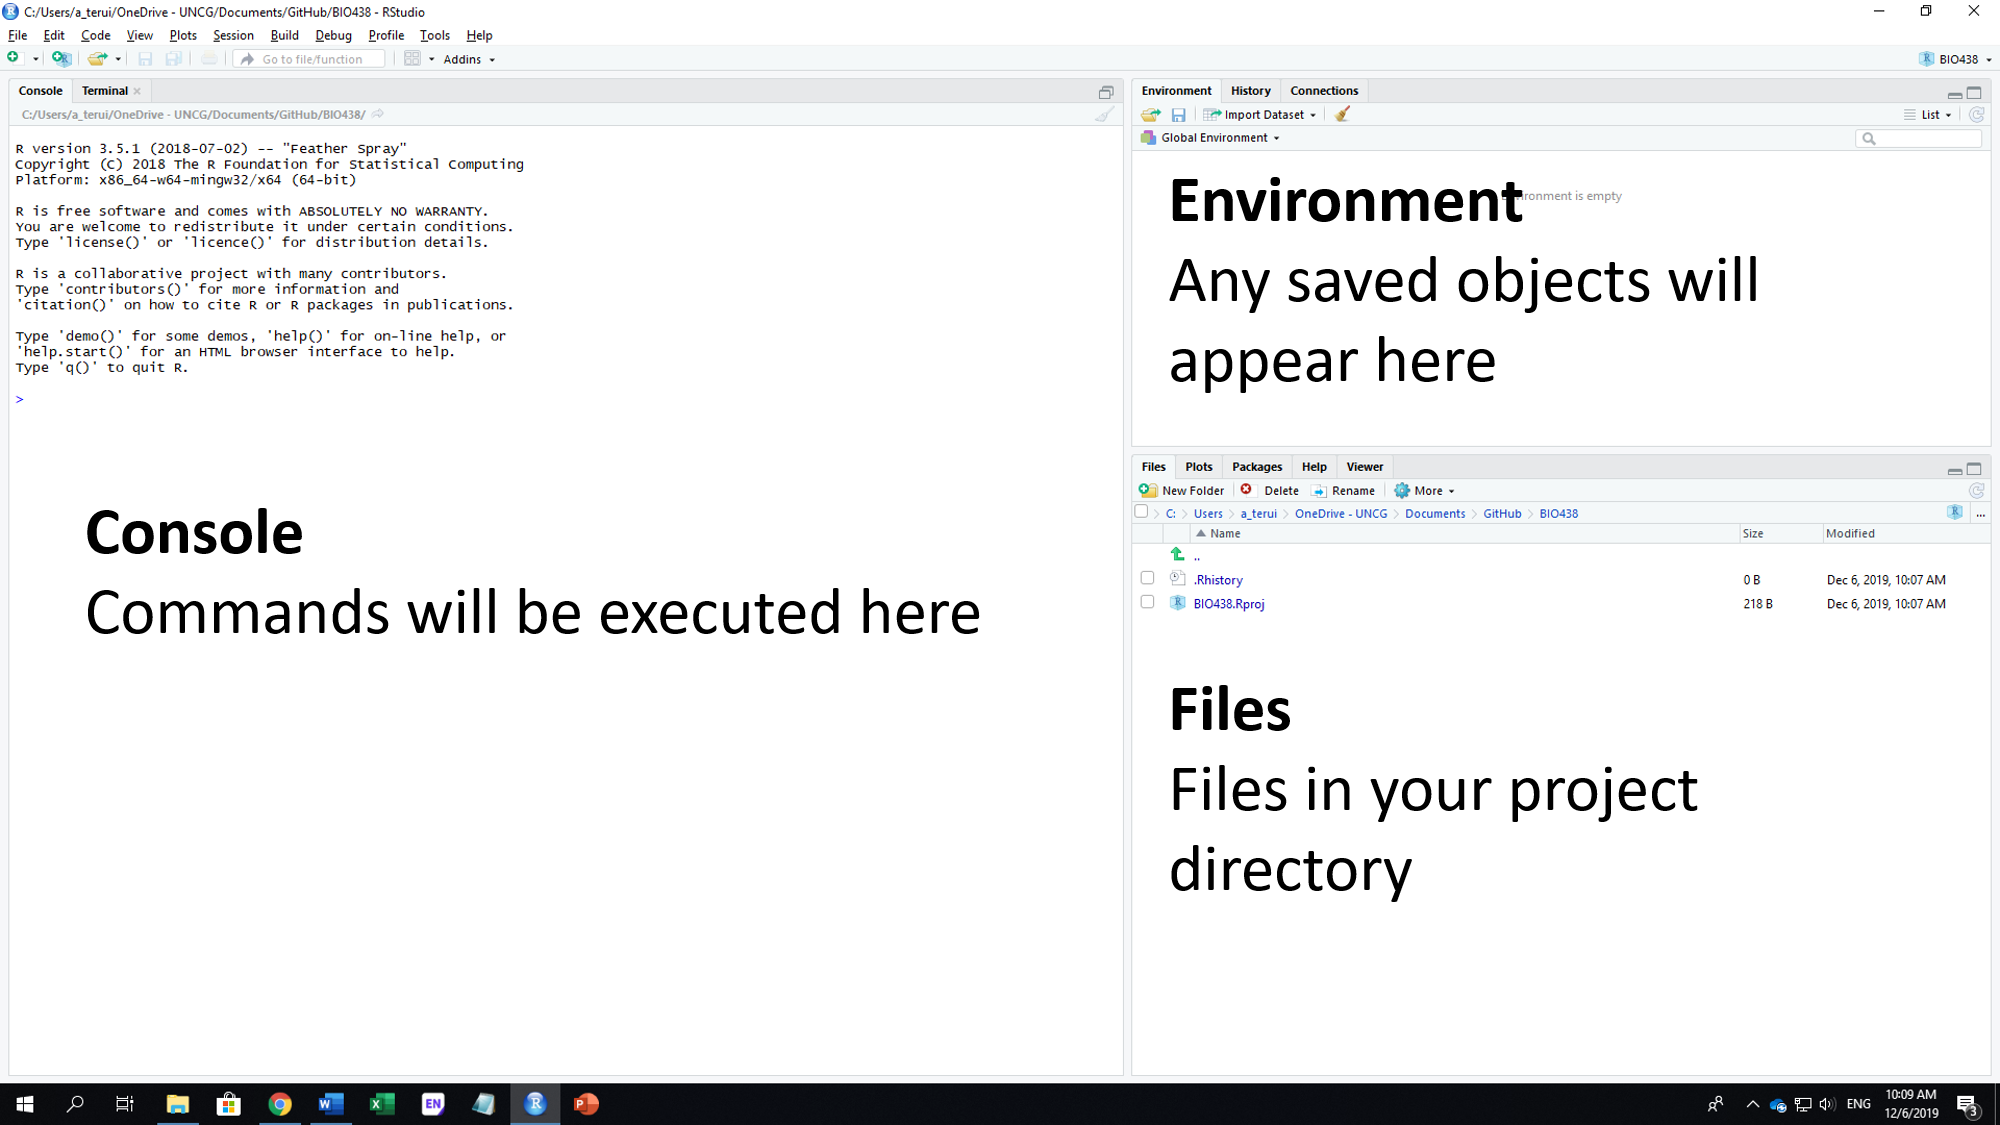
\includegraphics[width=27.78in]{image/r_image01} \caption{R Studio interface.}\label{fig:ui}
\end{figure}

Although you can work on your data as it appears, \textbf{it is actually a BAD idea}. As you work on your project, numerous materials will be generated. How do you manage files? If you randomly locate those materials within your computer, you will lose necessary items sooner or later. For this reason, I assemble all the relevant materials in a single \texttt{R\ Project}. You can create a new \texttt{R\ Project} with the following procedure.

\begin{enumerate}
\def\labelenumi{\alph{enumi}.}
\tightlist
\item
  Go to \texttt{File\ \textgreater{}\ New\ Project} on the top menu
\item
  Select \texttt{New\ Directory}
\item
  Select \texttt{New\ Project}
\end{enumerate}

A new window pops up and prompts you to name a directory with a location in your computer. Click \texttt{Browse} to select a location for the directory.

\textbf{IMPORTANT:} When you locate your project directories in your computer, I would strongly recommend to create a designated space. For example, in my computer, I have a folder named /\texttt{r\_project} in which all the \texttt{R\ Project} directories are located.

\hypertarget{internal-structure}{%
\section{Internal Structure}\label{internal-structure}}

The internal structure of an \texttt{R\ Project} is extremely important to navigate yourself (others once it's published). \texttt{R\ Project} will be composed of multiple types of files, typically \texttt{.R}, \texttt{.csv}, \texttt{.rds}, \texttt{.Rmd} among others. Unless those files are arranged in an organized manner, it is VERY LIKELY to make severe errors in coding. So take this seriously. Table \ref{tab:str} is my suggested subdirectory structure.

\begin{longtable}[]{@{}
  >{\raggedright\arraybackslash}p{(\columnwidth - 2\tabcolsep) * \real{0.2361}}
  >{\raggedright\arraybackslash}p{(\columnwidth - 2\tabcolsep) * \real{0.7639}}@{}}
\caption{\label{tab:str} Suggested internal structure of \texttt{R\ Project}}\tabularnewline
\toprule()
\begin{minipage}[b]{\linewidth}\raggedright
Name
\end{minipage} & \begin{minipage}[b]{\linewidth}\raggedright
Content
\end{minipage} \\
\midrule()
\endfirsthead
\toprule()
\begin{minipage}[b]{\linewidth}\raggedright
Name
\end{minipage} & \begin{minipage}[b]{\linewidth}\raggedright
Content
\end{minipage} \\
\midrule()
\endhead
\texttt{readme.md} & Markdown file explaining contents in the \texttt{R\ Project}. A derived file from \texttt{README.Rmd}. \\
\texttt{/code} & Sub-directory for R scripts (\texttt{.R}). \\
\texttt{/data\_raw} & Sub-directory for raw data before data manipulation (\texttt{.csv} or other formats). Files in this sub-directory MUST NOT be modified unless there are changes to raw data entries. \\
\texttt{/data\_format} & Sub-directory for formatted data (\texttt{.csv}, \texttt{.rds}, or other formats). \\
\texttt{/output} & Sub-directory for result outputs (\texttt{.csv}, \texttt{.rds}, or other formats). This may include statistical estimates from linear regression models etc. \\
\texttt{/rmd} & (Optional) Sub-directory for Rmarkdown files (\texttt{.Rmd}). Rmarkdown allows seamless integration of R scripts and text. \\
\bottomrule()
\end{longtable}

\hypertarget{file-name}{%
\section{File Name}\label{file-name}}

As you proceed, the number of files will increase, perhaps exponentially. It is therefore critical to have \textbf{consistent naming rules} for your files. Here are some recommendations:

\begin{itemize}
\tightlist
\item
  \textbf{NO SPACE.} Instead, use underscore or hyphen.

  \begin{itemize}
  \tightlist
  \item
    Do: \texttt{script\_week1.R} \texttt{script-week1.R}
  \item
    Don't: \texttt{script\ week1.R}
  \end{itemize}
\item
  \textbf{NO UPPERCASE.} Use lowercase only for file names.

  \begin{itemize}
  \tightlist
  \item
    Do: \texttt{script\_week1.R}
  \item
    Don't: \texttt{Script\_week1.R}
  \end{itemize}
\item
  \textbf{BE CONSISTENT.} Apply consistent naming rules within a project.

  \begin{itemize}
  \tightlist
  \item
    Do: R scripts for figures always start with a common prefix, e.g., \texttt{figure\_XXX.R} \texttt{figure\_YYY.R}(\texttt{XXX} and \texttt{YYY} specifies further details).
  \item
    Don't: R scripts for figures start with random text, e.g., \texttt{XXX\_fig.R} , \texttt{Figure\_Y2.R} , \texttt{plotB.R}.
  \end{itemize}
\end{itemize}

\hypertarget{data-structure}{%
\chapter{DATA STRUCTURE}\label{data-structure}}

\hypertarget{overview}{%
\section{Overview}\label{overview}}

R has 6 basic \textbf{data types}.

\begin{itemize}
\tightlist
\item
  character: \texttt{"aquatic"}, \texttt{"ecology"} (no order)
\item
  factor: similar to character, but has \emph{levels} (alphabetically ordered by default)
\item
  numeric: \texttt{20.0} , \texttt{15.5}
\item
  integer: \texttt{3}, \texttt{7}
\item
  logical: \texttt{TRUE} , \texttt{FALSE}
\item
  complex: \texttt{1+2i} (complex numbers with real and imaginary parts)
\end{itemize}

These elements form one of the following \textbf{data structures}.

\begin{itemize}
\tightlist
\item
  \textbf{vector}: a series of elements. A single data type is allowed in a single vector
\item
  \textbf{matrix}: elements organized into rows and columns. A single data type is allowed in a single matrix
\item
  \textbf{data frame}: looks similar to a matrix, but allows different data types in different columns
\end{itemize}

\hypertarget{vector}{%
\section{Vector}\label{vector}}

\hypertarget{create-vector}{%
\subsection{Create Vector}\label{create-vector}}

Below are examples of atomic character vectors, numeric vectors, integer vectors, etc. There are many ways to create vector data. The following examples use \texttt{c()}, \texttt{:}, \texttt{seq()}, \texttt{rep()}:

\begin{verbatim}
## [1] 1 3 4 8
\end{verbatim}

\begin{verbatim}
## [1] "a" "b" "c"
\end{verbatim}

\begin{verbatim}
## [1]  TRUE FALSE FALSE
\end{verbatim}

\begin{verbatim}
## [1] 1 2 3 4 5
\end{verbatim}

\begin{verbatim}
## [1] 2 2 2 2 2
\end{verbatim}

\begin{verbatim}
## [1] "a" "a" "a" "a" "a"
\end{verbatim}

\begin{verbatim}
## [1] 1 2 3 4 5
\end{verbatim}

\begin{verbatim}
##  [1] 1.0 1.1 1.2 1.3 1.4 1.5 1.6 1.7 1.8 1.9 2.0 2.1 2.2 2.3 2.4 2.5 2.6 2.7 2.8
## [20] 2.9 3.0 3.1 3.2 3.3 3.4 3.5 3.6 3.7 3.8 3.9 4.0 4.1 4.2 4.3 4.4 4.5 4.6 4.7
## [39] 4.8 4.9 5.0
\end{verbatim}

\hypertarget{check-features}{%
\subsection{Check Features}\label{check-features}}

R provides many functions to examine features of vectors and other objects, for example:

\begin{itemize}
\tightlist
\item
  \texttt{class()} - what kind of object (data structure) is it (high-level)?
\item
  \texttt{typeof()} - what is the object's data type (low-level)?
\item
  \texttt{attributes()} - does it have any metadata?
\item
  \texttt{length()} - how long is it? What about two dimensional objects?
\item
  \texttt{sum()} - what is the summed number of the data?
\item
  \texttt{mean()} - what is the average number of the data?
\end{itemize}

\textbf{Numeric Vector}

\begin{verbatim}
## [1] 1.2 3.1 4.0 8.2
\end{verbatim}

\begin{verbatim}
## [1] "numeric"
\end{verbatim}

\begin{verbatim}
## [1] "double"
\end{verbatim}

\begin{verbatim}
## [1] 4
\end{verbatim}

\begin{verbatim}
## [1] 16.5
\end{verbatim}

\begin{verbatim}
## [1] 4.125
\end{verbatim}

\textbf{Character Vector}

\begin{verbatim}
## [1] "character"
\end{verbatim}

\begin{verbatim}
## [1] 3
\end{verbatim}

\hypertarget{access}{%
\subsection{Access}\label{access}}

\textbf{Element ID}\\
Use brackets \texttt{{[}{]}} when accessing specific elements in an object. For example, if you want to access element \#2 in the vector \texttt{x}, you may specify as \texttt{x{[}2{]}}:

\begin{verbatim}
## [1] 2
\end{verbatim}

\begin{verbatim}
## [1] 2 2
\end{verbatim}

\begin{verbatim}
## [1] 2 3 2
\end{verbatim}

\textbf{Equation}\\
R provides many ways to access elements that suffice specific conditions. You can use mathematical symbols to specify what you need, for example:

\begin{itemize}
\tightlist
\item
  \texttt{==} equal
\item
  \texttt{\textgreater{}} larger than
\item
  \texttt{\textgreater{}=} equal \& larger than
\item
  \texttt{\textless{}} smaller than
\item
  \texttt{\textless{}=} equal \& smaller than
\item
  \texttt{which()} a function that returns element \# that suffices the specified condition
\end{itemize}

The following examples return a logical vector indicating whether each element in x suffices the specified condition:

\begin{verbatim}
## [1]  TRUE  TRUE FALSE  TRUE FALSE
\end{verbatim}

\begin{verbatim}
## [1] FALSE FALSE  TRUE FALSE  TRUE
\end{verbatim}

You can access elements that suffice the specified condition using brackets, for example:

\begin{verbatim}
## [1] 2 2 2
\end{verbatim}

\begin{verbatim}
## [1] 3 5
\end{verbatim}

Using \texttt{which()}, you can see which elements (i.e., \#) matches what you need:

\begin{verbatim}
## [1] 1 2 4
\end{verbatim}

\begin{verbatim}
## [1] 3 5
\end{verbatim}

\hypertarget{matrix}{%
\section{Matrix}\label{matrix}}

\hypertarget{create-matrix}{%
\subsection{Create Matrix}\label{create-matrix}}

Matrix is a set of elements (\emph{single data type}) that are organized into rows and columns:

\begin{verbatim}
##      [,1] [,2]
## [1,]    1    4
## [2,]    2    5
## [3,]    3    6
\end{verbatim}

\begin{verbatim}
##      [,1] [,2] [,3]
## [1,]    1    2    3
## [2,]    4    5    6
\end{verbatim}

\begin{verbatim}
##      [,1] [,2] [,3]
## [1,]    1    4    7
## [2,]    2    5    8
## [3,]    3    6    9
\end{verbatim}

\hypertarget{check-features-1}{%
\subsection{Check Features}\label{check-features-1}}

R provides many functions to examine features of matrix data, for example:

\begin{itemize}
\tightlist
\item
  \texttt{class()} what kind of object (data type) is it (high-level)?
\item
  \texttt{typeof()} what is the object's data type (low-level)?
\item
  \texttt{attributes()} does it have any metadata?
\item
  \texttt{dim()} how long are rows and columns?
\item
  \texttt{rowSums()} what is the summed number of the data for each row?
\item
  \texttt{colSums()} what is the summed number of the data for each column?
\end{itemize}

\textbf{Integer Matrix}\\

\begin{verbatim}
##      [,1] [,2] [,3]
## [1,]    1    4    7
## [2,]    2    5    8
## [3,]    3    6    9
\end{verbatim}

\begin{verbatim}
## [1] "matrix" "array"
\end{verbatim}

\begin{verbatim}
## [1] "integer"
\end{verbatim}

\begin{verbatim}
## [1] 3 3
\end{verbatim}

\textbf{Character Matrix}\\

\begin{verbatim}
##      [,1] [,2]
## [1,] "a"  "d" 
## [2,] "b"  "e" 
## [3,] "c"  "f"
\end{verbatim}

\begin{verbatim}
## [1] "matrix" "array"
\end{verbatim}

\begin{verbatim}
## [1] "character"
\end{verbatim}

\begin{verbatim}
## [1] 3 2
\end{verbatim}

\hypertarget{access-1}{%
\subsection{Access}\label{access-1}}

When accessing matrix elements, you need to pick row(s) and/or column(s), for example:

\begin{verbatim}
##      [,1] [,2] [,3]
## [1,]    1    4    7
## [2,]    2    5    8
## [3,]    3    6    9
\end{verbatim}

\begin{verbatim}
## [1] 8
\end{verbatim}

\begin{verbatim}
## [1] 2 5 8
\end{verbatim}

\begin{verbatim}
##      [,1] [,2] [,3]
## [1,]    2    5    8
## [2,]    3    6    9
\end{verbatim}

\begin{verbatim}
##      [,1] [,2]
## [1,]    4    7
## [2,]    5    8
## [3,]    6    9
\end{verbatim}

You can assess each element with mathematical expressions just like vectors:

\begin{verbatim}
##       [,1]  [,2]  [,3]
## [1,] FALSE FALSE FALSE
## [2,]  TRUE FALSE FALSE
## [3,] FALSE FALSE FALSE
\end{verbatim}

\begin{verbatim}
##       [,1] [,2] [,3]
## [1,] FALSE TRUE TRUE
## [2,] FALSE TRUE TRUE
## [3,]  TRUE TRUE TRUE
\end{verbatim}

However, care must be taken when accessing elements, as it will be automatically converted to vector data:

\begin{verbatim}
## [1] 2
\end{verbatim}

\begin{verbatim}
## [1] 3 4 5 6 7 8 9
\end{verbatim}

\texttt{which()} needs an additional argument to return both row and column \#:

\begin{verbatim}
##      row col
## [1,]   2   1
\end{verbatim}

\begin{verbatim}
##      row col
## [1,]   3   1
## [2,]   1   2
## [3,]   2   2
## [4,]   3   2
## [5,]   1   3
## [6,]   2   3
## [7,]   3   3
\end{verbatim}

\hypertarget{data-frame}{%
\section{Data Frame}\label{data-frame}}

Data frame is a set of elements that are organized into rows and columns, but differ from matrix in several ways.

\begin{itemize}
\tightlist
\item
  it allows \emph{multiple data types} in different columns
\item
  each column has its \emph{name}
\item
  you can access columns by name (using \texttt{\$})
\end{itemize}

\textbf{Data frame is the most common data structure when manipulating ecological data}. A data set loaded from a spread sheet (we will address this later) will be automatically recognized as a data frame. Here is an example:

\textbf{Create a data frame}\\
In the following example, variables \texttt{x} and \texttt{y} are organized into a single data frame \texttt{dat}. Variable are renamed when creating a data frame composed of \texttt{x} and \texttt{y}.

\begin{verbatim}
##    LakeType  TSS
## 1  Pristine  1.2
## 2  Pristine  2.2
## 3 Disturbed 10.9
## 4 Disturbed 50.0
## 5  Pristine  3.0
\end{verbatim}

\textbf{Call column names}\\

\begin{verbatim}
## [1] "LakeType" "TSS"
\end{verbatim}

\textbf{Access by columns}\\

\begin{verbatim}
## [1] "Pristine"  "Pristine"  "Disturbed" "Disturbed" "Pristine"
\end{verbatim}

\begin{verbatim}
## [1]  1.2  2.2 10.9 50.0  3.0
\end{verbatim}

You can access elements like a matrix as well:

\begin{verbatim}
## [1] "Pristine"  "Pristine"  "Disturbed" "Disturbed" "Pristine"
\end{verbatim}

\begin{verbatim}
##   LakeType TSS
## 1 Pristine 1.2
\end{verbatim}

\begin{verbatim}
##    LakeType  TSS
## 2  Pristine  2.2
## 4 Disturbed 50.0
\end{verbatim}

\hypertarget{exercise}{%
\section{Exercise}\label{exercise}}

Download a template (R script file).

\hypertarget{vector-1}{%
\subsection{Vector}\label{vector-1}}

\begin{enumerate}
\def\labelenumi{\alph{enumi}.}
\tightlist
\item
  Create three numeric vectors with length 3, 6 and 20, respectively. Each vector must be created using different functions in R.
\item
  Create three character vectors with length 3, 6 and 20, respectively. Each vector must be created using different functions in R.
\item
  Copy the following script to your R script and perform the following analysis:
\end{enumerate}

\begin{itemize}
\tightlist
\item
  Identify element IDs of \texttt{x} that are greater than \texttt{2.0}
\item
  Identify element values of \texttt{x} that are greater than \texttt{2.0}
\end{itemize}

\hypertarget{matrix-1}{%
\subsection{Matrix}\label{matrix-1}}

\begin{enumerate}
\def\labelenumi{\alph{enumi}.}
\tightlist
\item
  Create a numeric matrix with 4 rows and 4 columns. Each column must contain identical elements.
\item
  Create a numeric matrix with 4 rows and 4 columns. Each row must contain identical elements.
\item
  Create a character matrix with 4 rows and 4 columns. Each column must contain identical elements.
\item
  Create a character matrix with 4 rows and 4 columns. Each row must contain identical elements.
\item
  Copy the following script to your R script and perform the following analysis:
\end{enumerate}

\begin{itemize}
\tightlist
\item
  Identify element IDs of \texttt{x} that are greater than \texttt{2.0} (\textbf{specify row and column IDs})
\item
  Identify element values of \texttt{x} that are greater than \texttt{2.0} and calculate the mean.
\end{itemize}

\hypertarget{data-frame-1}{%
\subsection{Data Frame}\label{data-frame-1}}

\begin{enumerate}
\def\labelenumi{\alph{enumi}.}
\tightlist
\item
  Create a data frame of 3 variables with 10 elements (name variables as \texttt{x}, \texttt{y} and \texttt{z}. \texttt{x} must be \texttt{character} while \texttt{y} and \texttt{z} must be \texttt{numeric}.
\item
  Check the data structure (higher-level) of \texttt{x}, \texttt{y} and \texttt{z}
\item
  Copy the following script to your R script and perform the following analysis:
\end{enumerate}

\begin{itemize}
\tightlist
\item
  Calculate the means of \texttt{temperature} and \texttt{abundance} for states \texttt{VA} and \texttt{NC} separately - use \texttt{tapply()} function
\end{itemize}

\hypertarget{visualization}{%
\chapter{VISUALIZATION}\label{visualization}}

\hypertarget{overview-1}{%
\section{Overview}\label{overview-1}}

R has a number of functions that help visualize data. \texttt{graphics} provides R functions for base graphics (\href{https://www.rdocumentation.org/packages/graphics/versions/3.6.2}{list of functions}). I will use \texttt{iris}, the built-in data set in R, to show how \texttt{graphics} functions work.

\begin{verbatim}
##     Sepal.Length Sepal.Width Petal.Length Petal.Width    Species
## 1            5.1         3.5          1.4         0.2     setosa
## 2            4.9         3.0          1.4         0.2     setosa
## 3            4.7         3.2          1.3         0.2     setosa
## 4            4.6         3.1          1.5         0.2     setosa
## 5            5.0         3.6          1.4         0.2     setosa
## 6            5.4         3.9          1.7         0.4     setosa
## 7            4.6         3.4          1.4         0.3     setosa
## 8            5.0         3.4          1.5         0.2     setosa
## 9            4.4         2.9          1.4         0.2     setosa
## 10           4.9         3.1          1.5         0.1     setosa
## 11           5.4         3.7          1.5         0.2     setosa
## 12           4.8         3.4          1.6         0.2     setosa
## 13           4.8         3.0          1.4         0.1     setosa
## 14           4.3         3.0          1.1         0.1     setosa
## 15           5.8         4.0          1.2         0.2     setosa
## 16           5.7         4.4          1.5         0.4     setosa
## 17           5.4         3.9          1.3         0.4     setosa
## 18           5.1         3.5          1.4         0.3     setosa
## 19           5.7         3.8          1.7         0.3     setosa
## 20           5.1         3.8          1.5         0.3     setosa
## 21           5.4         3.4          1.7         0.2     setosa
## 22           5.1         3.7          1.5         0.4     setosa
## 23           4.6         3.6          1.0         0.2     setosa
## 24           5.1         3.3          1.7         0.5     setosa
## 25           4.8         3.4          1.9         0.2     setosa
## 26           5.0         3.0          1.6         0.2     setosa
## 27           5.0         3.4          1.6         0.4     setosa
## 28           5.2         3.5          1.5         0.2     setosa
## 29           5.2         3.4          1.4         0.2     setosa
## 30           4.7         3.2          1.6         0.2     setosa
## 31           4.8         3.1          1.6         0.2     setosa
## 32           5.4         3.4          1.5         0.4     setosa
## 33           5.2         4.1          1.5         0.1     setosa
## 34           5.5         4.2          1.4         0.2     setosa
## 35           4.9         3.1          1.5         0.2     setosa
## 36           5.0         3.2          1.2         0.2     setosa
## 37           5.5         3.5          1.3         0.2     setosa
## 38           4.9         3.6          1.4         0.1     setosa
## 39           4.4         3.0          1.3         0.2     setosa
## 40           5.1         3.4          1.5         0.2     setosa
## 41           5.0         3.5          1.3         0.3     setosa
## 42           4.5         2.3          1.3         0.3     setosa
## 43           4.4         3.2          1.3         0.2     setosa
## 44           5.0         3.5          1.6         0.6     setosa
## 45           5.1         3.8          1.9         0.4     setosa
## 46           4.8         3.0          1.4         0.3     setosa
## 47           5.1         3.8          1.6         0.2     setosa
## 48           4.6         3.2          1.4         0.2     setosa
## 49           5.3         3.7          1.5         0.2     setosa
## 50           5.0         3.3          1.4         0.2     setosa
## 51           7.0         3.2          4.7         1.4 versicolor
## 52           6.4         3.2          4.5         1.5 versicolor
## 53           6.9         3.1          4.9         1.5 versicolor
## 54           5.5         2.3          4.0         1.3 versicolor
## 55           6.5         2.8          4.6         1.5 versicolor
## 56           5.7         2.8          4.5         1.3 versicolor
## 57           6.3         3.3          4.7         1.6 versicolor
## 58           4.9         2.4          3.3         1.0 versicolor
## 59           6.6         2.9          4.6         1.3 versicolor
## 60           5.2         2.7          3.9         1.4 versicolor
## 61           5.0         2.0          3.5         1.0 versicolor
## 62           5.9         3.0          4.2         1.5 versicolor
## 63           6.0         2.2          4.0         1.0 versicolor
## 64           6.1         2.9          4.7         1.4 versicolor
## 65           5.6         2.9          3.6         1.3 versicolor
## 66           6.7         3.1          4.4         1.4 versicolor
## 67           5.6         3.0          4.5         1.5 versicolor
## 68           5.8         2.7          4.1         1.0 versicolor
## 69           6.2         2.2          4.5         1.5 versicolor
## 70           5.6         2.5          3.9         1.1 versicolor
## 71           5.9         3.2          4.8         1.8 versicolor
## 72           6.1         2.8          4.0         1.3 versicolor
## 73           6.3         2.5          4.9         1.5 versicolor
## 74           6.1         2.8          4.7         1.2 versicolor
## 75           6.4         2.9          4.3         1.3 versicolor
## 76           6.6         3.0          4.4         1.4 versicolor
## 77           6.8         2.8          4.8         1.4 versicolor
## 78           6.7         3.0          5.0         1.7 versicolor
## 79           6.0         2.9          4.5         1.5 versicolor
## 80           5.7         2.6          3.5         1.0 versicolor
## 81           5.5         2.4          3.8         1.1 versicolor
## 82           5.5         2.4          3.7         1.0 versicolor
## 83           5.8         2.7          3.9         1.2 versicolor
## 84           6.0         2.7          5.1         1.6 versicolor
## 85           5.4         3.0          4.5         1.5 versicolor
## 86           6.0         3.4          4.5         1.6 versicolor
## 87           6.7         3.1          4.7         1.5 versicolor
## 88           6.3         2.3          4.4         1.3 versicolor
## 89           5.6         3.0          4.1         1.3 versicolor
## 90           5.5         2.5          4.0         1.3 versicolor
## 91           5.5         2.6          4.4         1.2 versicolor
## 92           6.1         3.0          4.6         1.4 versicolor
## 93           5.8         2.6          4.0         1.2 versicolor
## 94           5.0         2.3          3.3         1.0 versicolor
## 95           5.6         2.7          4.2         1.3 versicolor
## 96           5.7         3.0          4.2         1.2 versicolor
## 97           5.7         2.9          4.2         1.3 versicolor
## 98           6.2         2.9          4.3         1.3 versicolor
## 99           5.1         2.5          3.0         1.1 versicolor
## 100          5.7         2.8          4.1         1.3 versicolor
## 101          6.3         3.3          6.0         2.5  virginica
## 102          5.8         2.7          5.1         1.9  virginica
## 103          7.1         3.0          5.9         2.1  virginica
## 104          6.3         2.9          5.6         1.8  virginica
## 105          6.5         3.0          5.8         2.2  virginica
## 106          7.6         3.0          6.6         2.1  virginica
## 107          4.9         2.5          4.5         1.7  virginica
## 108          7.3         2.9          6.3         1.8  virginica
## 109          6.7         2.5          5.8         1.8  virginica
## 110          7.2         3.6          6.1         2.5  virginica
## 111          6.5         3.2          5.1         2.0  virginica
## 112          6.4         2.7          5.3         1.9  virginica
## 113          6.8         3.0          5.5         2.1  virginica
## 114          5.7         2.5          5.0         2.0  virginica
## 115          5.8         2.8          5.1         2.4  virginica
## 116          6.4         3.2          5.3         2.3  virginica
## 117          6.5         3.0          5.5         1.8  virginica
## 118          7.7         3.8          6.7         2.2  virginica
## 119          7.7         2.6          6.9         2.3  virginica
## 120          6.0         2.2          5.0         1.5  virginica
## 121          6.9         3.2          5.7         2.3  virginica
## 122          5.6         2.8          4.9         2.0  virginica
## 123          7.7         2.8          6.7         2.0  virginica
## 124          6.3         2.7          4.9         1.8  virginica
## 125          6.7         3.3          5.7         2.1  virginica
## 126          7.2         3.2          6.0         1.8  virginica
## 127          6.2         2.8          4.8         1.8  virginica
## 128          6.1         3.0          4.9         1.8  virginica
## 129          6.4         2.8          5.6         2.1  virginica
## 130          7.2         3.0          5.8         1.6  virginica
## 131          7.4         2.8          6.1         1.9  virginica
## 132          7.9         3.8          6.4         2.0  virginica
## 133          6.4         2.8          5.6         2.2  virginica
## 134          6.3         2.8          5.1         1.5  virginica
## 135          6.1         2.6          5.6         1.4  virginica
## 136          7.7         3.0          6.1         2.3  virginica
## 137          6.3         3.4          5.6         2.4  virginica
## 138          6.4         3.1          5.5         1.8  virginica
## 139          6.0         3.0          4.8         1.8  virginica
## 140          6.9         3.1          5.4         2.1  virginica
## 141          6.7         3.1          5.6         2.4  virginica
## 142          6.9         3.1          5.1         2.3  virginica
## 143          5.8         2.7          5.1         1.9  virginica
## 144          6.8         3.2          5.9         2.3  virginica
## 145          6.7         3.3          5.7         2.5  virginica
## 146          6.7         3.0          5.2         2.3  virginica
## 147          6.3         2.5          5.0         1.9  virginica
## 148          6.5         3.0          5.2         2.0  virginica
## 149          6.2         3.4          5.4         2.3  virginica
## 150          5.9         3.0          5.1         1.8  virginica
\end{verbatim}

\hypertarget{plot}{%
\section{\texorpdfstring{\texttt{plot()}}{plot()}}\label{plot}}

When plotting data, what's you need is to specify the \textbf{formula}. For example, if you want to visualize the relationship between \texttt{x} and \texttt{y} (\texttt{y} on the vertical axis and \texttt{x} on the horizontal axis), the formula would be \texttt{y\ \textasciitilde{}\ x} (the left side of the formula will be on the vertical axis). In the \texttt{iris} data set, the following columns are available: \texttt{Sepal.Length} \texttt{Sepal.Width} \texttt{Petal.Length} \texttt{Petal.Width} \texttt{Species}. In the following example, the relationship between \texttt{Sepal.Length} and \texttt{Sepal.Width} is plotted:

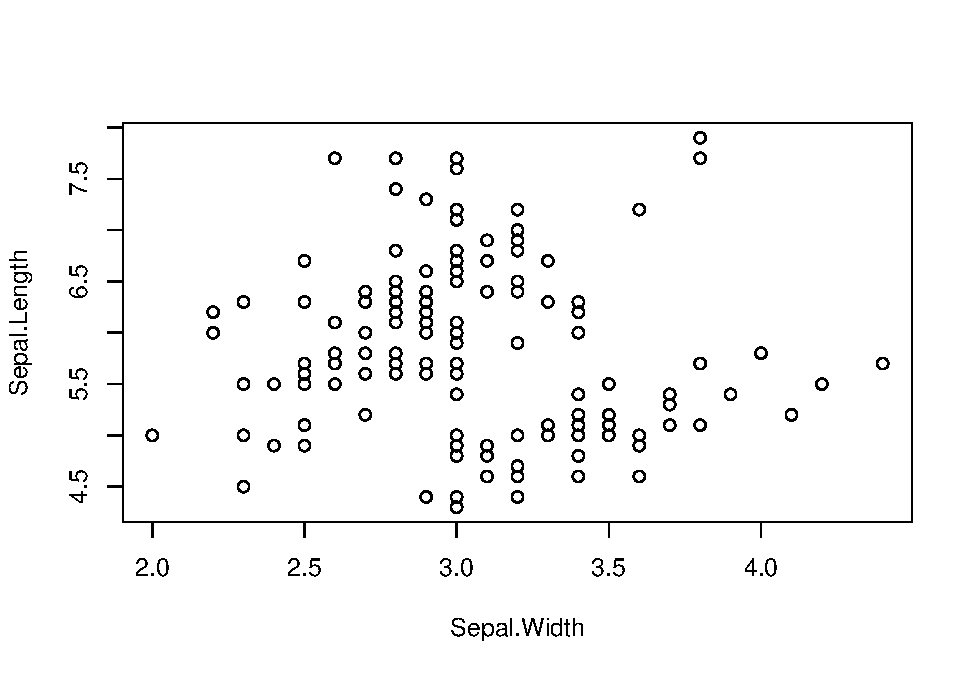
\includegraphics{_main_files/figure-latex/unnamed-chunk-23-1.pdf}

The argument \texttt{data\ =} tells the function the data set from which the variables (\texttt{Sepal.Length} and \texttt{Sepal.Width}) are extracted. The above figure is the default setting, and you may customize it as necessary. Below is an example of how you may customize:

\hypertarget{symbol}{%
\subsection{Symbol}\label{symbol}}

\texttt{pch} argument. Choose from \texttt{1} to \texttt{25} (google \textbf{r plot pch} for details)

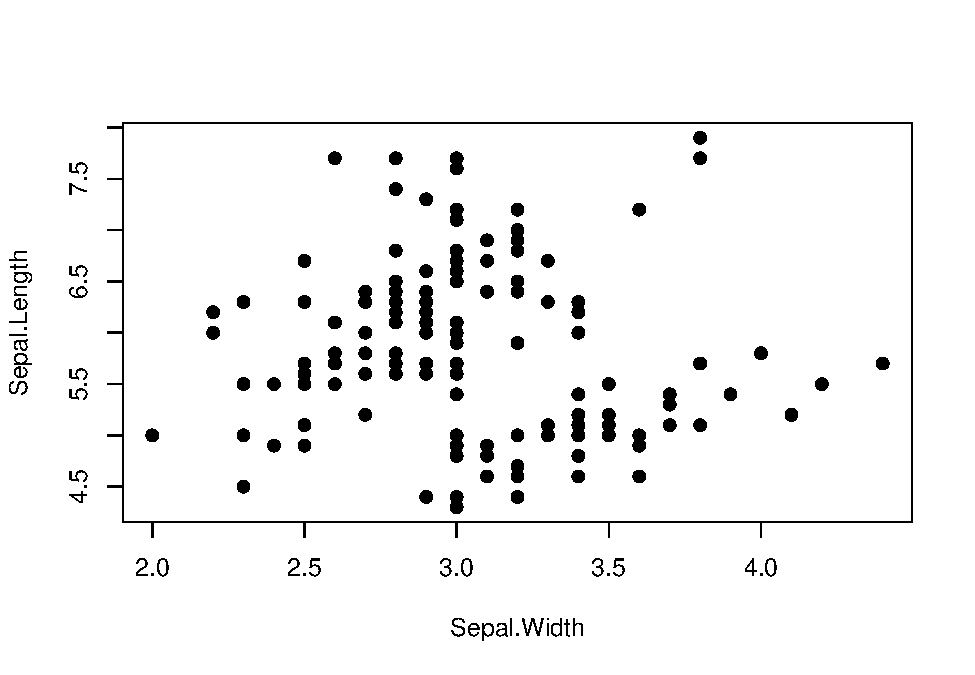
\includegraphics{_main_files/figure-latex/unnamed-chunk-24-1.pdf}

\hypertarget{symbol-size}{%
\subsection{Symbol size}\label{symbol-size}}

\texttt{cex} argument. \texttt{cex\ =\ 1} is the default value. \texttt{cex\ =\ 2} is as twice large as default value.

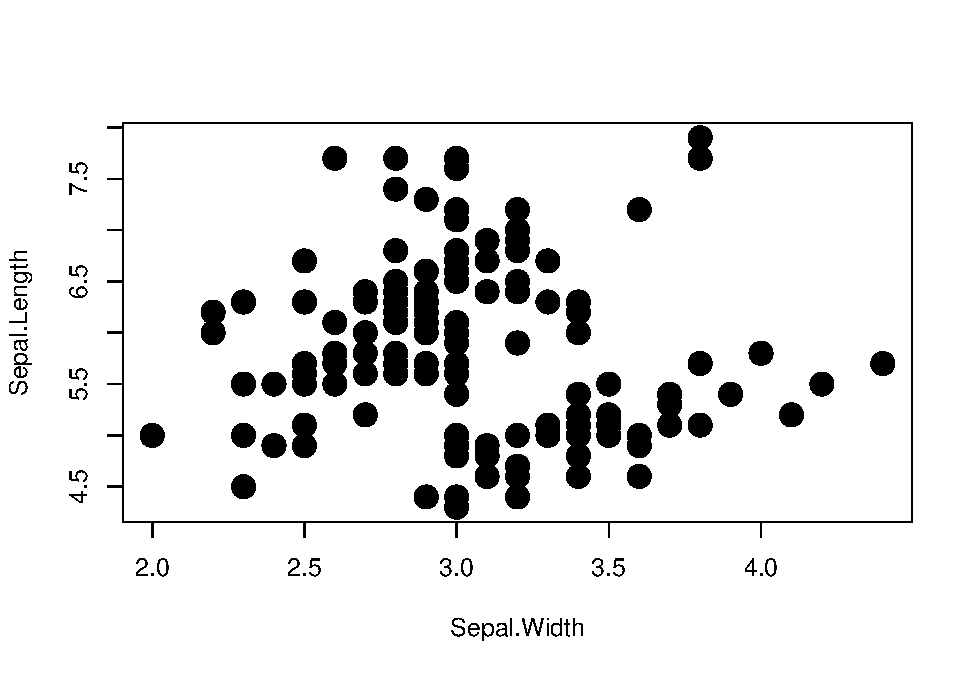
\includegraphics{_main_files/figure-latex/unnamed-chunk-25-1.pdf}

\hypertarget{symbol-color-border}{%
\subsection{Symbol color (border)}\label{symbol-color-border}}

\texttt{col} argument (quote \texttt{"color\ name"} when specifying). Google \textbf{r color name} for color options.

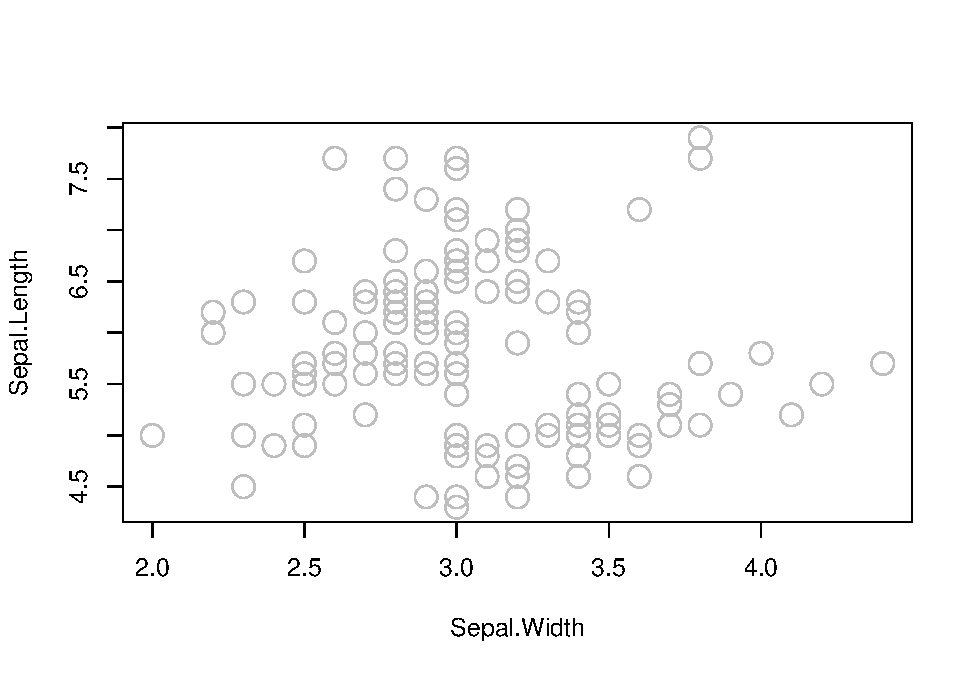
\includegraphics{_main_files/figure-latex/unnamed-chunk-26-1.pdf}

\hypertarget{symbol-color-fill}{%
\subsection{Symbol color (fill)}\label{symbol-color-fill}}

\texttt{bg} argument (quote \texttt{"color\ name"} when specifying). Available for a subset of symbol options (some symbols have pre-defined filled color).

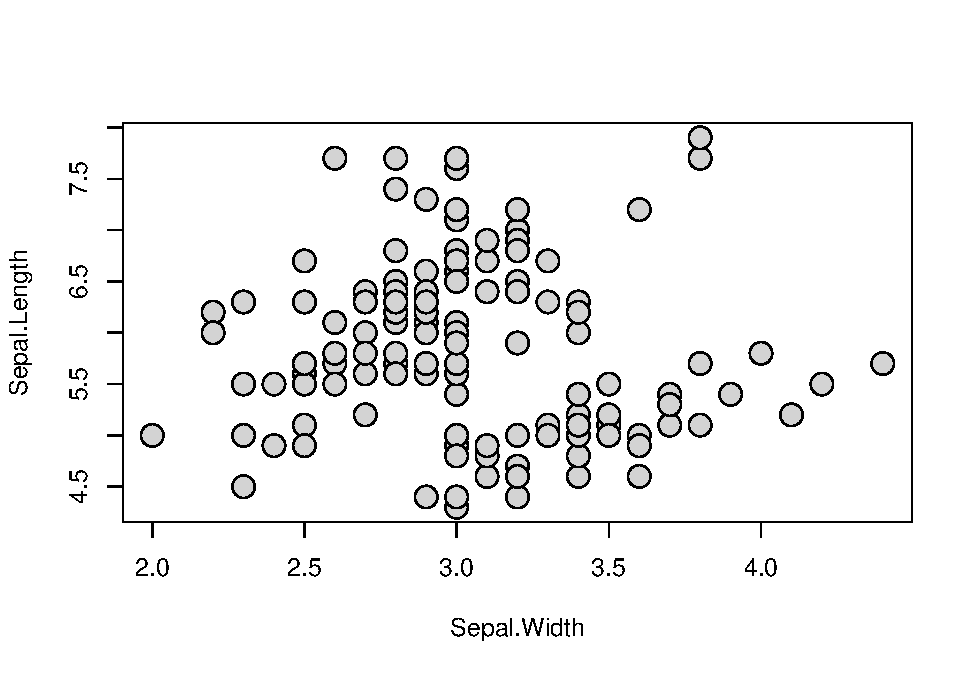
\includegraphics{_main_files/figure-latex/unnamed-chunk-27-1.pdf}

\hypertarget{label}{%
\subsection{Label}\label{label}}

\texttt{ylab} or \texttt{xlab} arguments. Provide \texttt{"quoted\ text"}.

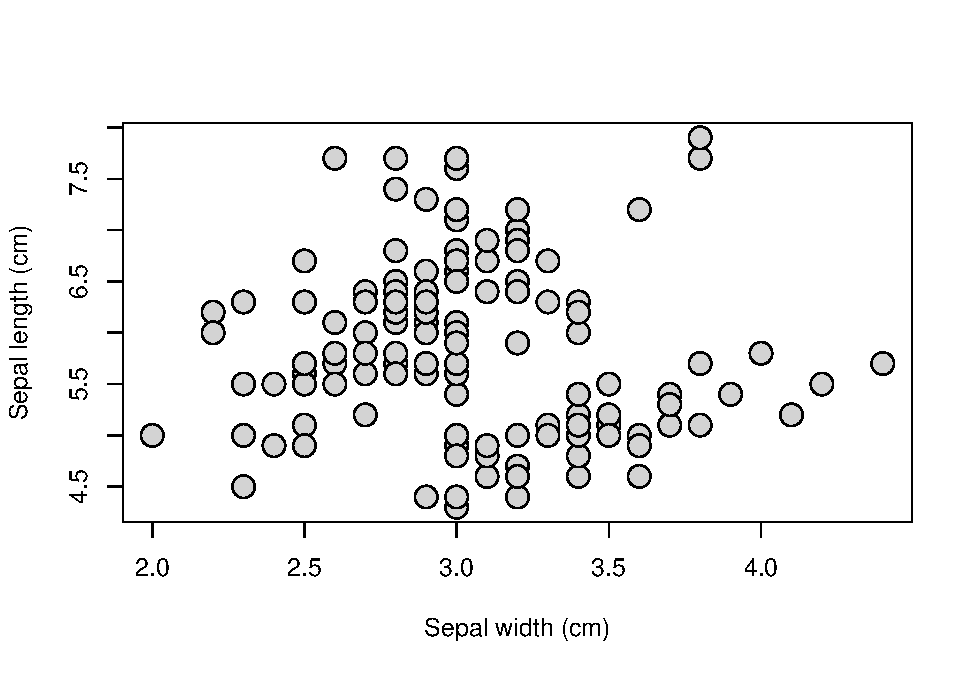
\includegraphics{_main_files/figure-latex/unnamed-chunk-28-1.pdf}

\hypertarget{axis}{%
\subsection{Axis}\label{axis}}

Delete axes with \texttt{axes\ =\ F} and re-draw with \texttt{box()} and \texttt{axis()} functions.

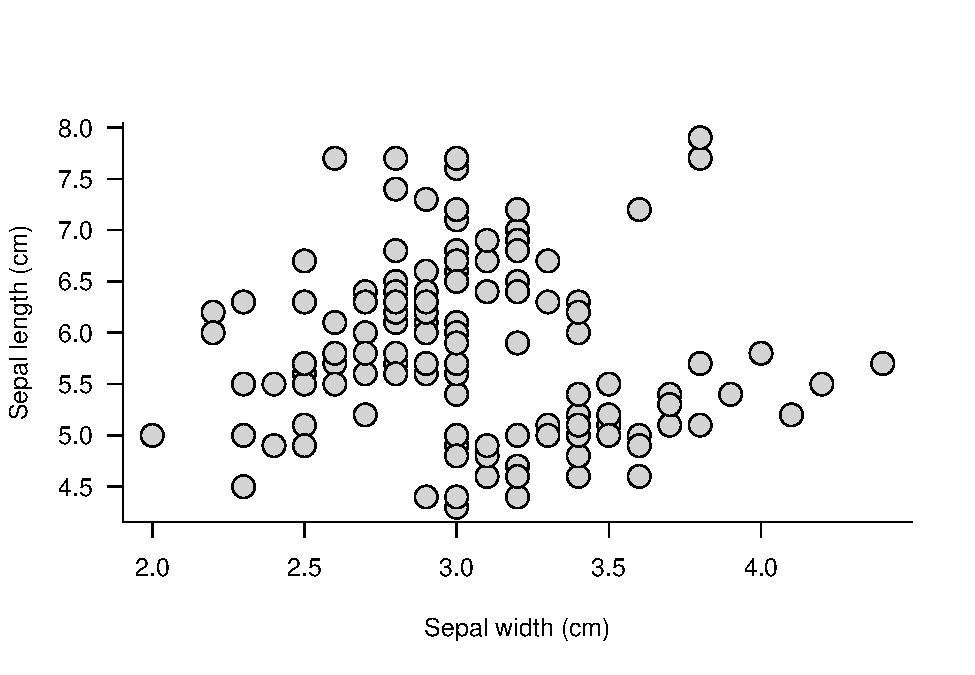
\includegraphics{_main_files/figure-latex/unnamed-chunk-29-1.pdf}

\hypertarget{boxplot}{%
\section{\texorpdfstring{\texttt{boxplot()}}{boxplot()}}\label{boxplot}}

\texttt{boxplot()} is used when the x-axis is factor-type data (by default, \texttt{plot()} will produce a boxplot when x-axis is a factor variable). In the \texttt{iris} dataset, the column \texttt{Species} is a factor variable. Compare \texttt{Sepal.Length} among species using \texttt{boxplot()}.

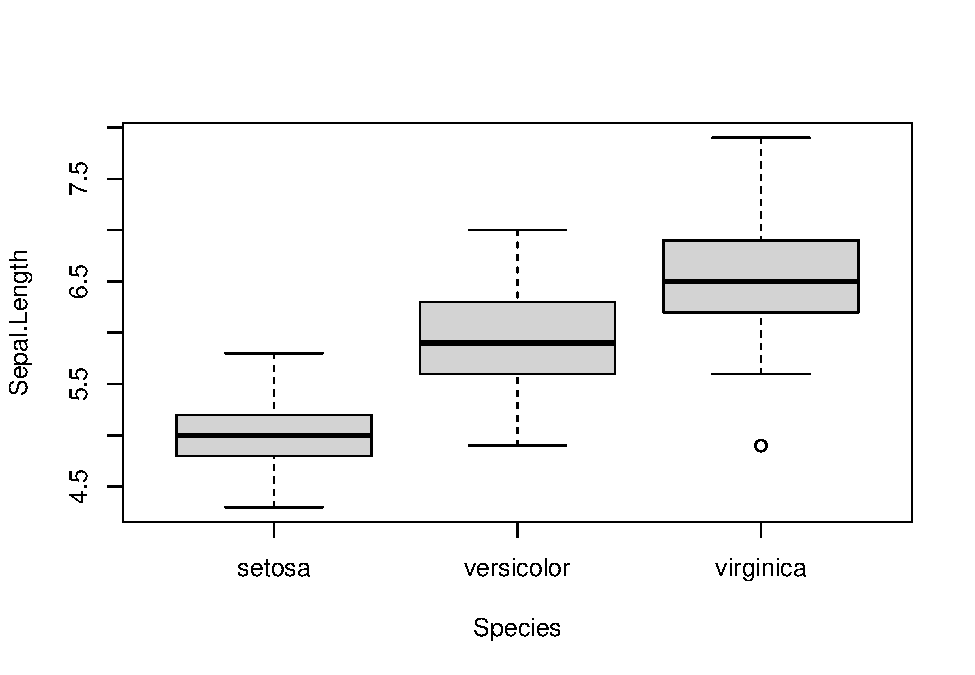
\includegraphics{_main_files/figure-latex/unnamed-chunk-30-1.pdf}

You can customize as in \texttt{plot()}, but slighlty different.

\hypertarget{box-color}{%
\subsection{Box color}\label{box-color}}

\texttt{col} argument.

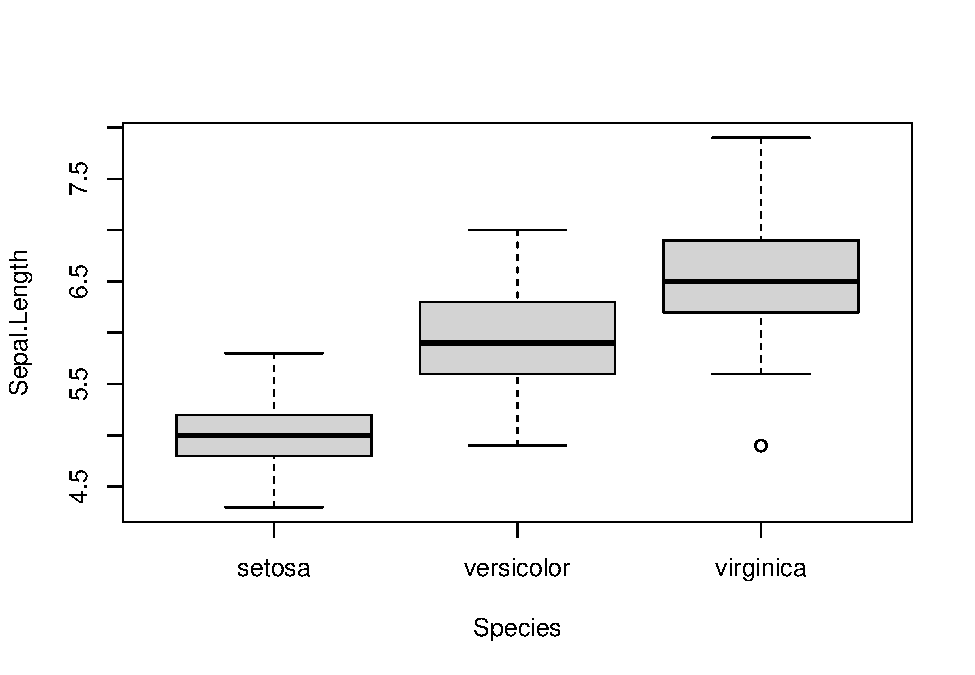
\includegraphics{_main_files/figure-latex/unnamed-chunk-31-1.pdf}

\hypertarget{border-color}{%
\subsection{Border color}\label{border-color}}

\texttt{border} argument.

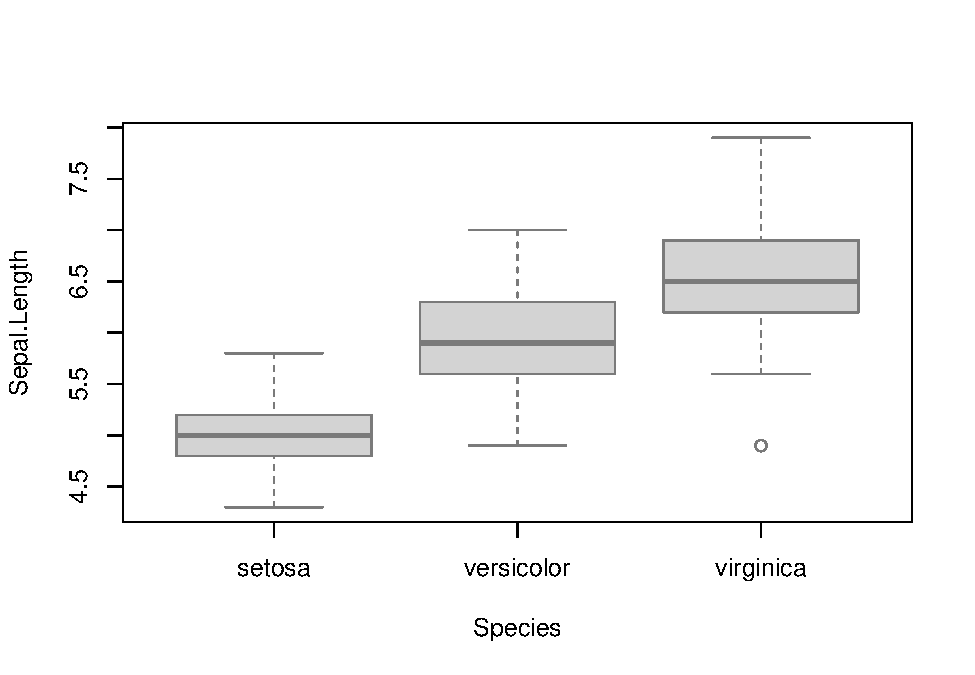
\includegraphics{_main_files/figure-latex/unnamed-chunk-32-1.pdf}

\hypertarget{box-width}{%
\subsection{Box width}\label{box-width}}

\texttt{boxwex} argument.

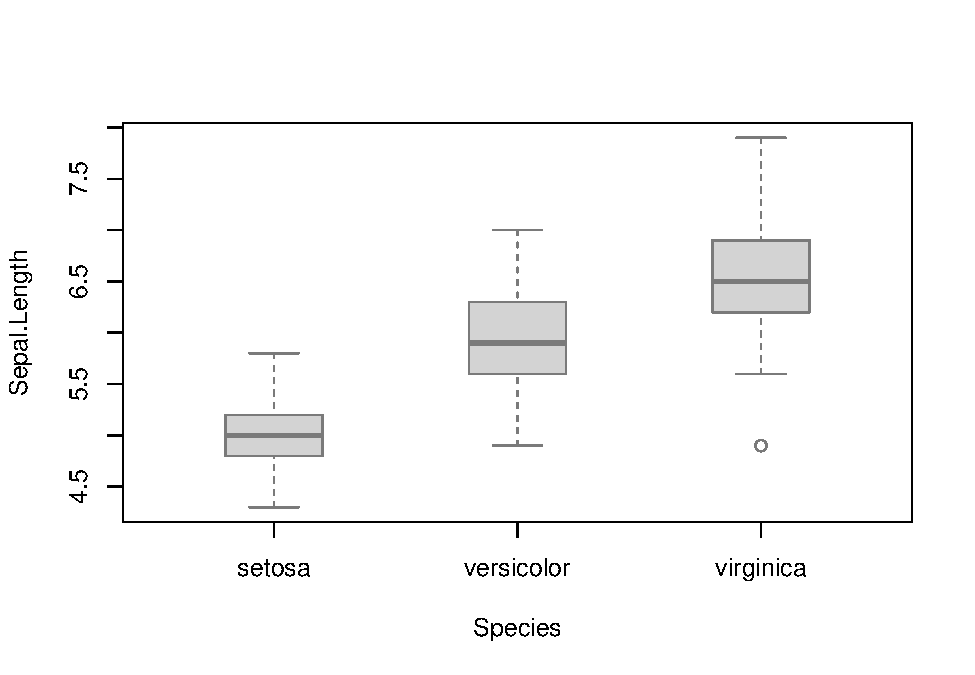
\includegraphics{_main_files/figure-latex/unnamed-chunk-33-1.pdf}

\hypertarget{axis-1}{%
\subsection{Axis}\label{axis-1}}

Delete axes with \texttt{axes\ =\ F} and re-draw with \texttt{box()} and \texttt{axis()} functions.

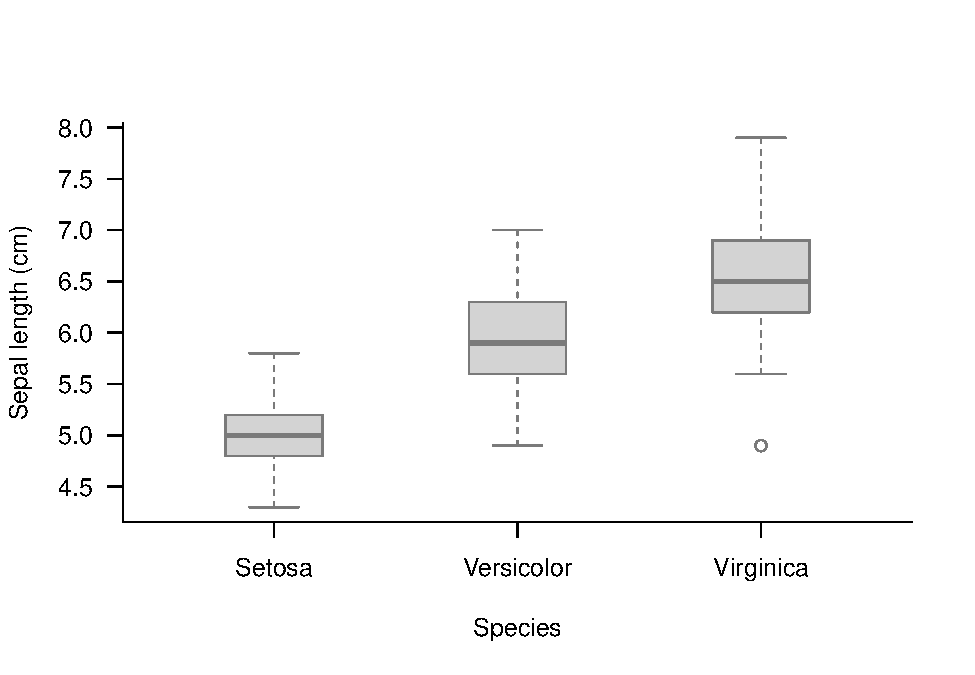
\includegraphics{_main_files/figure-latex/unnamed-chunk-34-1.pdf}

\hypertarget{exercise-1}{%
\section{Exercise}\label{exercise-1}}

Download a template (R script file).

\hypertarget{plot-function}{%
\subsection{\texorpdfstring{\texttt{plot()} function}{plot() function}}\label{plot-function}}

\begin{enumerate}
\def\labelenumi{\alph{enumi}.}
\tightlist
\item
  Plot the relationship between \texttt{Sepal.Width} and \texttt{Petal.Width}
\item
  Turn symbol color (border) into red.
\item
  Turn symbol color (fill) into red (set \texttt{pch\ =\ 21}).
\item
  Make symbol size larger.
\item
  Make L-shaped plot border (delete border lines on upper and right sides)
\end{enumerate}

\hypertarget{boxplot-function}{%
\subsection{\texorpdfstring{\texttt{boxplot()} function}{boxplot() function}}\label{boxplot-function}}

\begin{enumerate}
\def\labelenumi{\alph{enumi}.}
\tightlist
\item
  Plot the relationship between \texttt{Petal.Width} and \texttt{Species}.
\item
  Turn box color (border) into \texttt{blue}.
\item
  Make box width narrower.
\end{enumerate}

  \bibliography{book.bib,packages.bib}

\end{document}
